
\begin{figure}[ht]
\centering
\begin{subfigure}{0.23\linewidth}
  \centering
  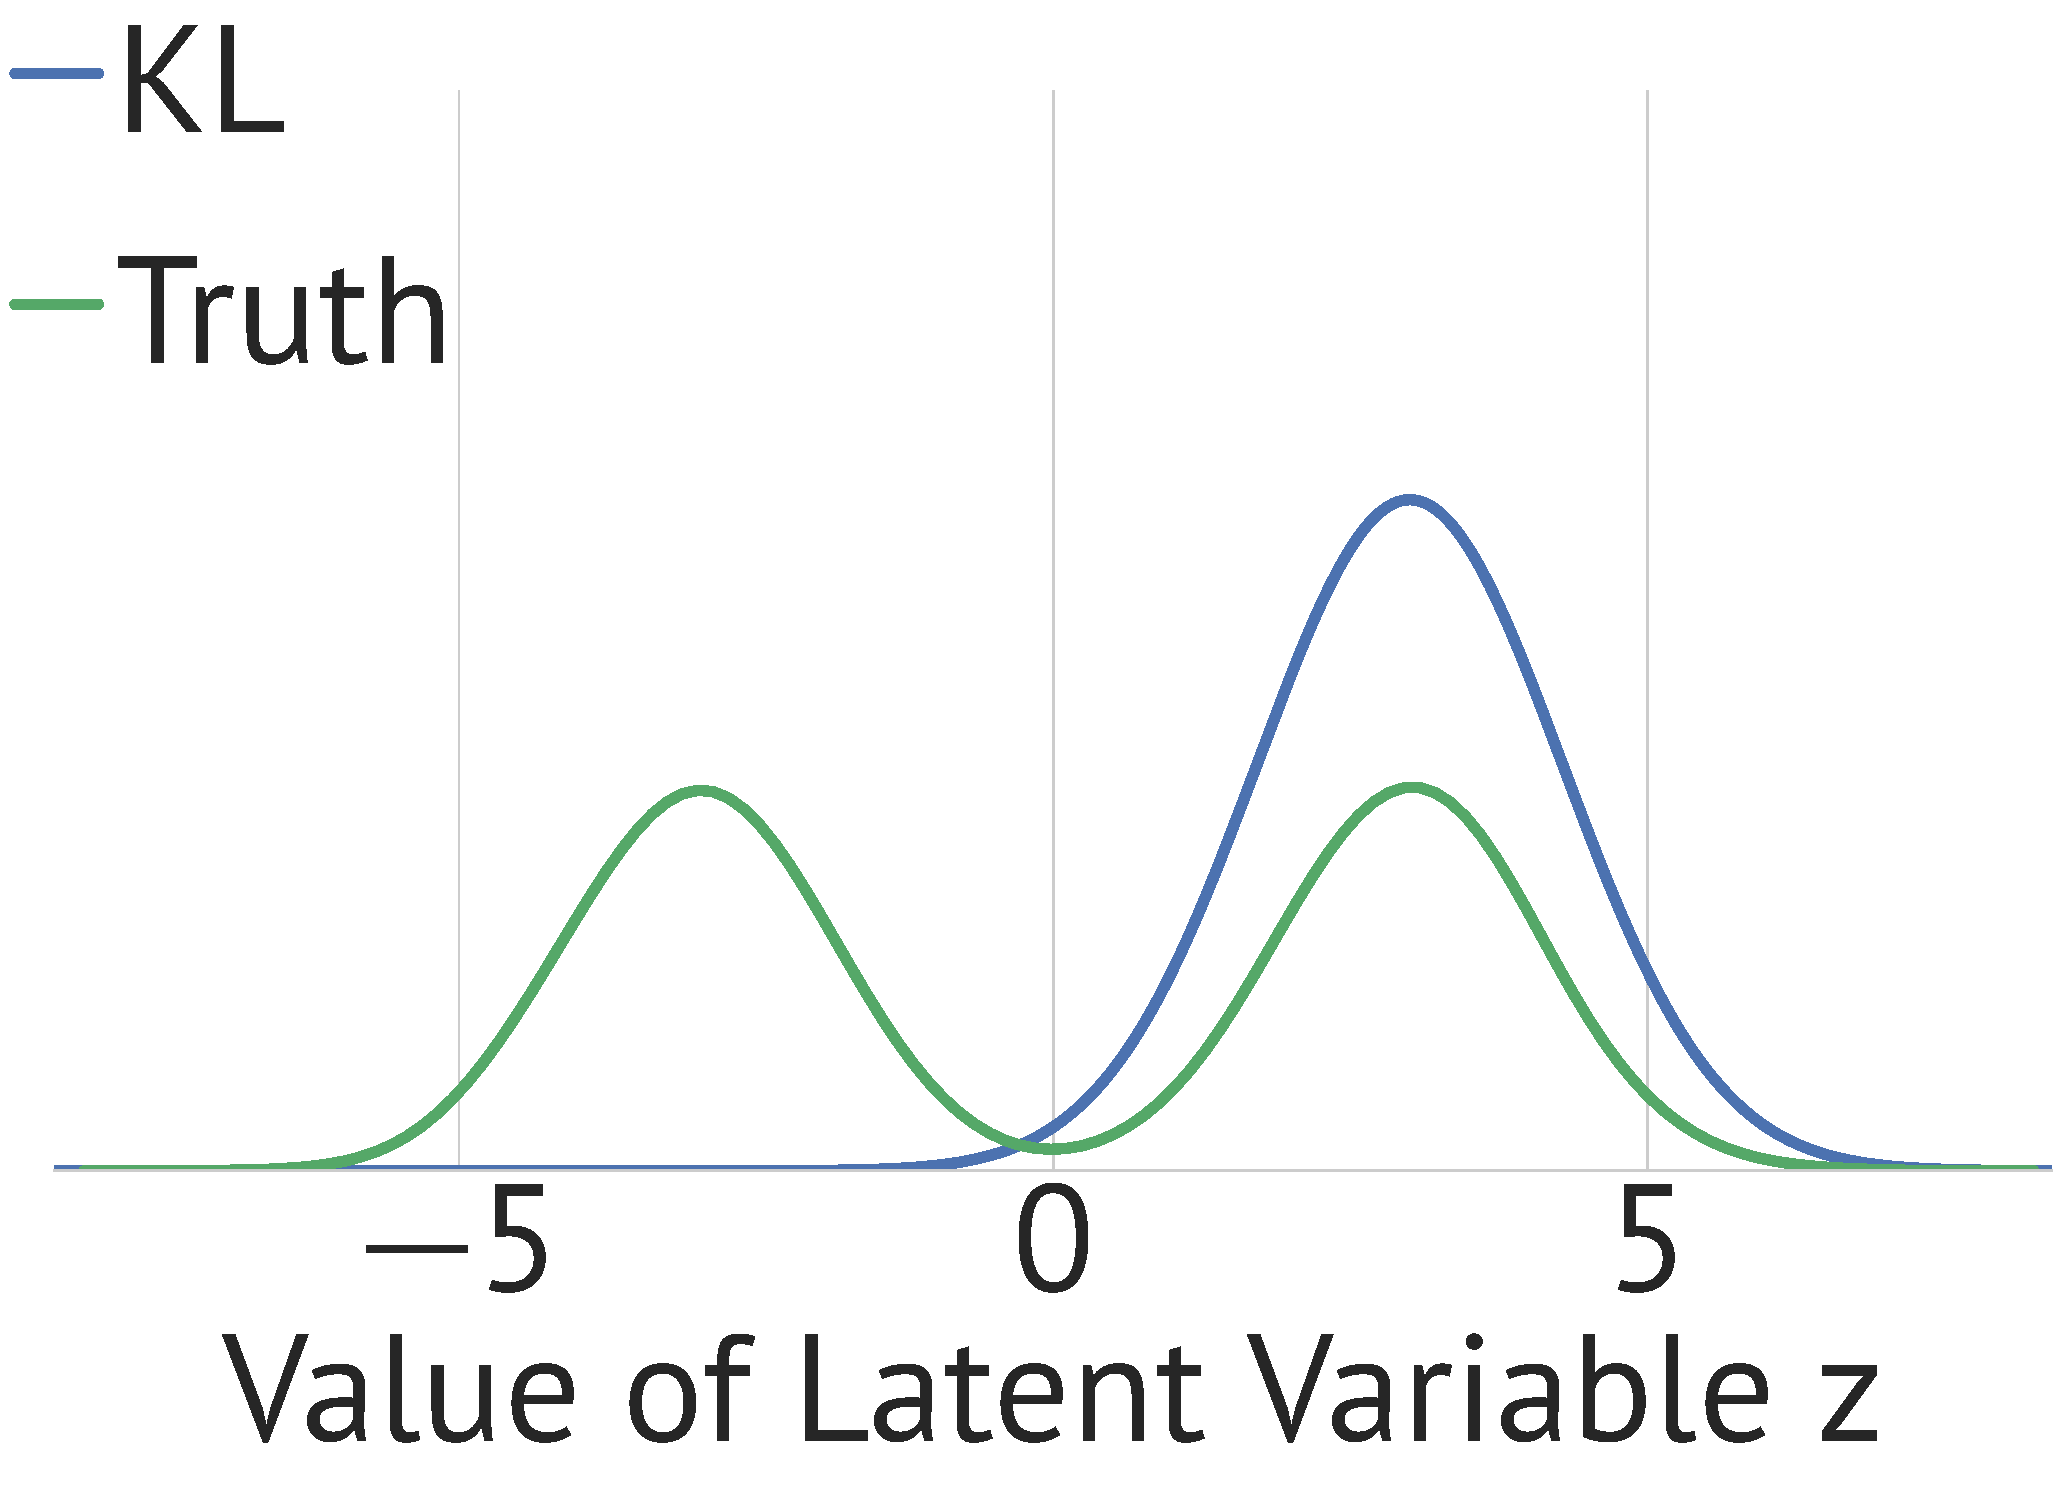
\includegraphics[trim=0 0 0 0, width=\linewidth]{fig/density_KL}
\end{subfigure}
\begin{subfigure}{0.23\textwidth}
  \centering
  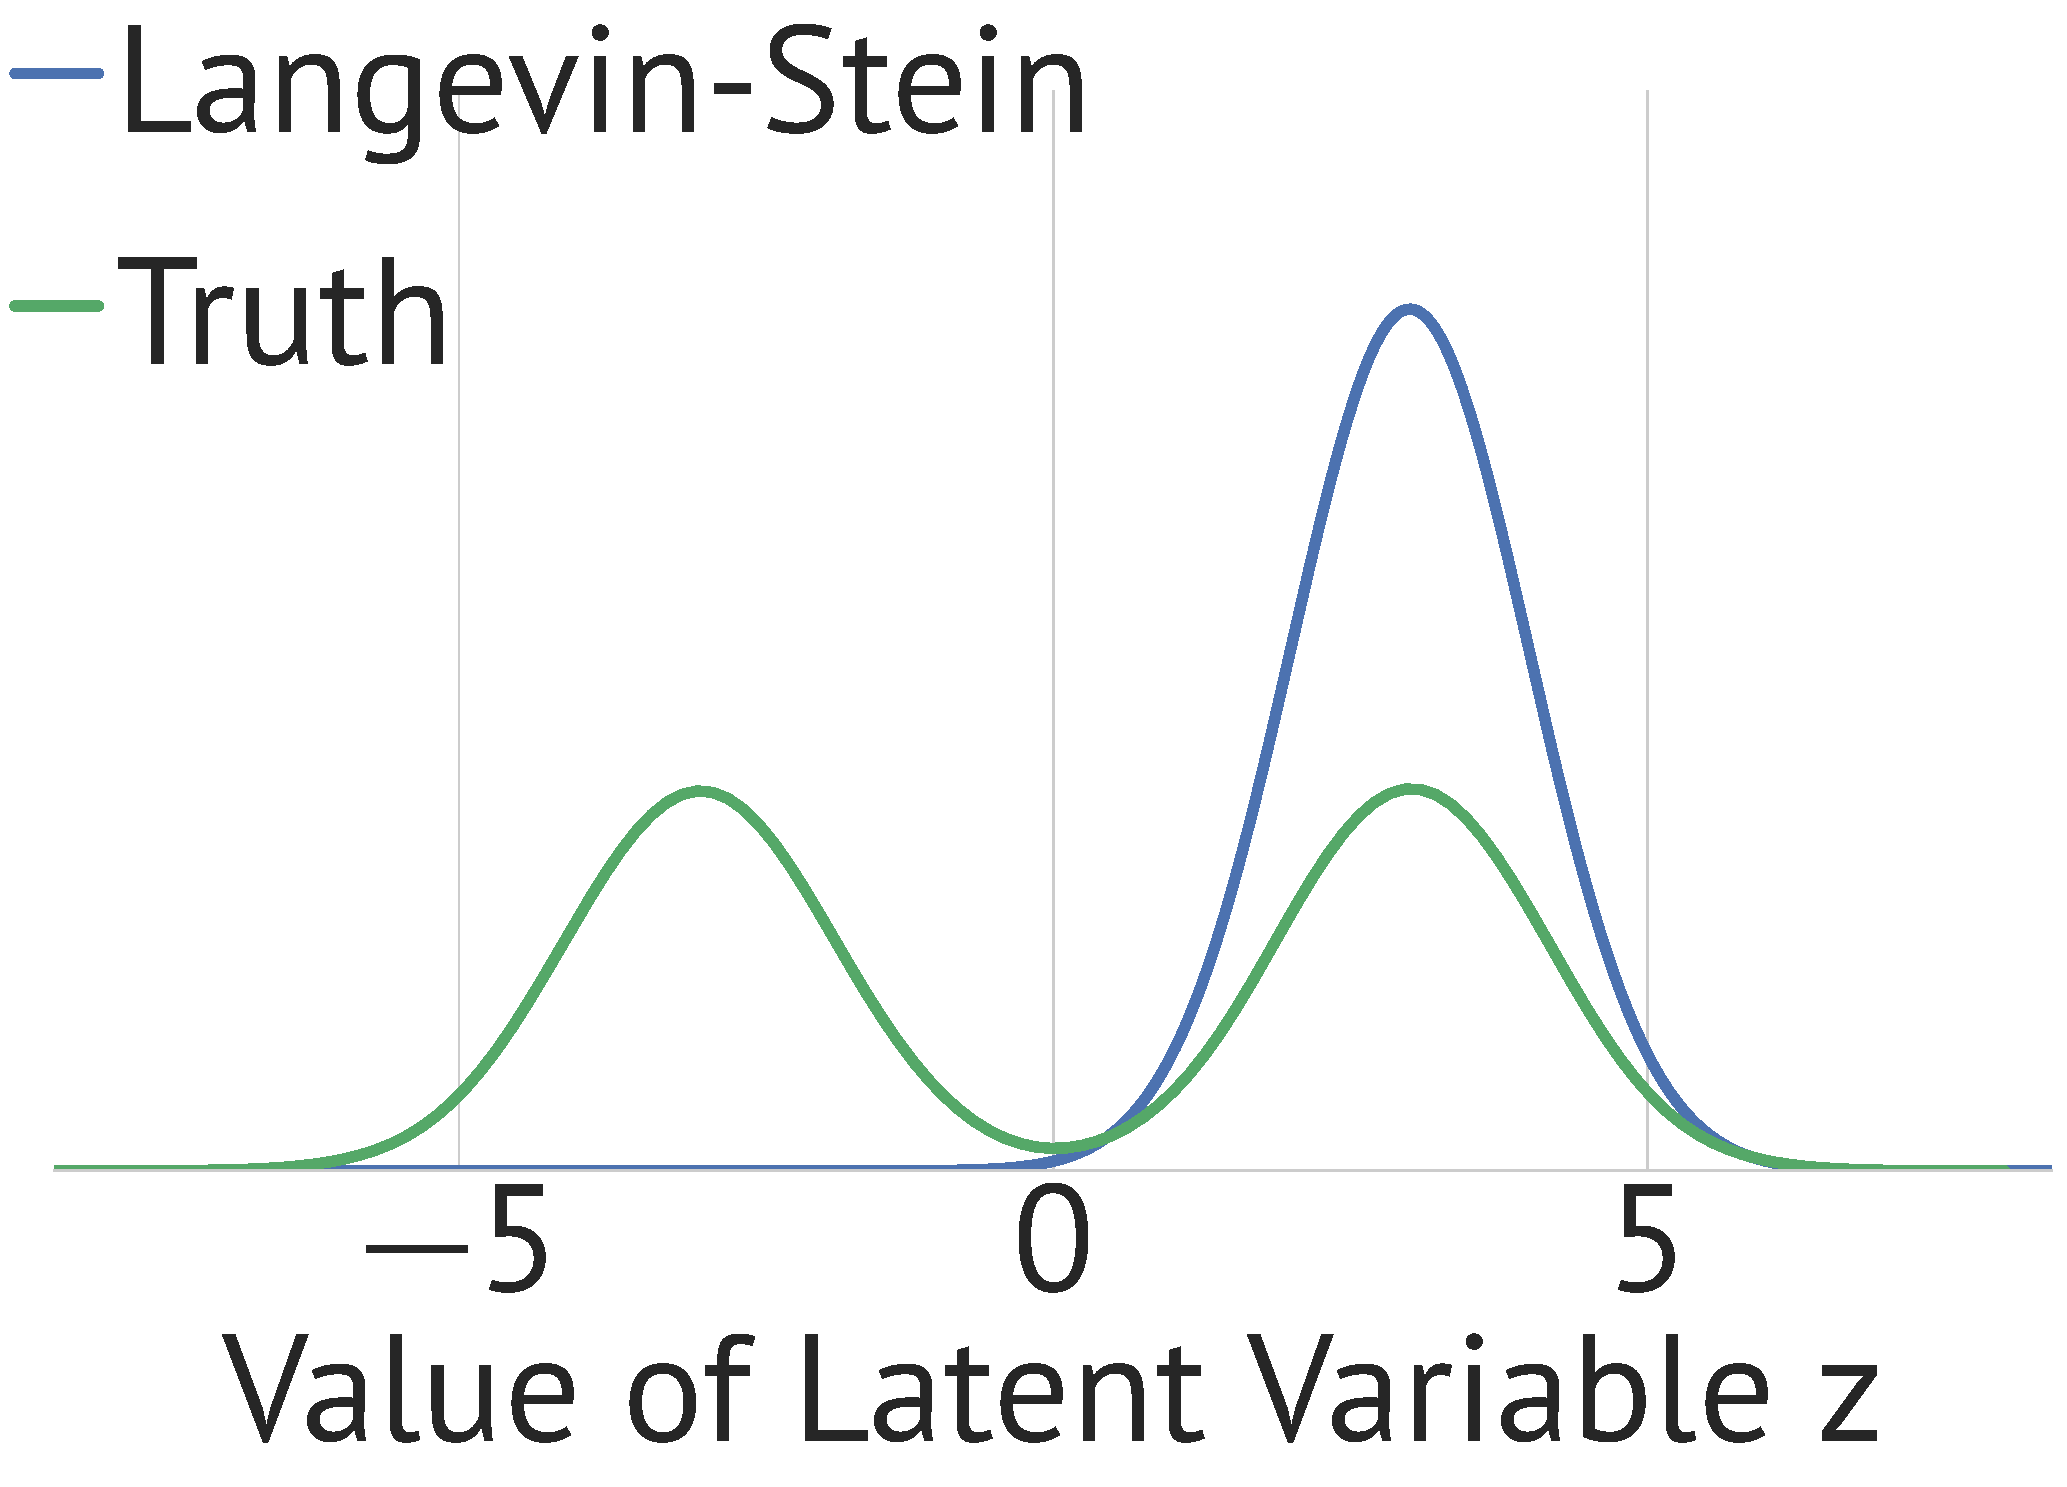
\includegraphics[trim=0 0 0 0, width=\linewidth]{fig/density_Lang-Stein}
\end{subfigure}
\begin{subfigure}{0.23\textwidth}
    \centering
   \includegraphics[trim=0 0 0 0, width=\linewidth]{{"fig/density_Variational Program"}}
\end{subfigure}
\caption{The true posterior is a mixture of two Gaussians, in green. We approximate it with
  a Gaussian using two operators (in blue). The density on the far
  right is a variational program given in~\Cref{eq:toy_var_prog} and
  using the Langevin-Stein operator; it approximates the truth well.
  The density of the variational program is intractable. We plot a histogram
  of its samples and compare this to the histogram of the true posterior.}
\label{fig:mog}\label{fig:toy}
\end{figure}
